% TODO: ensure all references in paper.bib are cited in the paper!
% TODO: format checklist (see e-mail)
\documentclass{acm_proc_article-sp}

\usepackage{pslatex}
\usepackage{epsfig}
\usepackage{appendix}
\usepackage{float}
\usepackage{url}

\floatstyle{ruled}
\newfloat{program}{thp}{lop}
\floatname{program}{Program}

\begin{document}

\title{Evaluation of Cache-Oblivious Data Structures}
\subtitle{\textit{Work In Progress!}}

\numberofauthors{1}
\author{Maks Verver\\ \email{m.verver@student.utwente.nl}}

% Obligatory permission block
\toappear{
Permission to make digital or hard copies of all or part of this work
for personal or classroom use is granted without fee provided that
copies are not made or distributed for profit or commercial advantage
and that copies bear this notice and the full citation on the first
page. To copy otherwise, or republish, to post on servers or to
redistribute to lists, requires prior specific permission.

\textit{\small 9$^{th}$ Twente Student Conference on IT, Enschede, June, 2008}

Copyright 2008, University of Twente, Faculty of Electrical Engineering,
Mathematics and Computer Science}
% End of obligatory permission block

\maketitle

\begin{abstract}
% TODO: rewrite (NB: max. 10 lines)
%In modern computer hardware architecture, memory is organized in a hierarchy
%consisting of several types of memory with different memory sizes, block
%transfer sizes and access times. The cache-oblivious model has been proposed
%to reflect this reality more accurately than traditional models. A number of
%algorithms and data structures have been proposed that perform optimally in
%this model. The goal of the proposed research project is to implement a
%selection of cache-oblivious set-like data structures, evaluate their
%performance (in terms of execution time and memory use) in a realistic
%environment, and compare their performance to traditional data structures.
\end{abstract}

% TODO: update keywords?
\keywords{cache efficiency, locality of reference, algorithms}

% TODO: more meaningful section titles?

\section{Introduction}
A fundamental part of theoretical computer science is the study of algorithms (formal descriptions of how computations may be performed) and data structures (descriptions of how information is organized and stored in computers). Traditionally, algorithms have been evaluated in a simplified model of computation. In this model it is assumed that a computer executes an algorithm in discrete steps. At each step it performs one elementary operation (e.g. comparing two numbers, adding one to another, storing a value in memory, et cetera). Each elementary operation is performed within a constant time. In this model, both storing and retrieving data values in memory is considered to be an elementary operation.

This model is close enough to the way computers work to be extremely useful in the development and analysis of data structures and algorithms that work well in practice. However, like every model, it is a simplification of reality. One of the simplifications is the assumption that storing and retrieving data in memory is a constant-time operation (i.e. the uniform memory model). Advancements in software and hardware design over the last two de\-cades have caused this assumption to be increasingly detached from reality.

One of the reasons this assumption fails is that modern operating systems employ virtual memory management, which allows (slower) disk-based storage to be dynamically substituted for (fast\-er) main memory when the latter is in short supply. Another reason is that as processor speeds have increased greatly, the time required to transfer data between processor and main memory has become a bottleneck for many types of computations. Hardware architects have added faster (but small) cache memory at various points in the computer architecture to reduce this problem, but this increases the differences in access time between different types of memory.

As a result, a modern computer system lacks a central memory storage with uniform performance characteristics. Instead, it employs a hierarchy of memory storage types. Figure \ref{fig-memhier} gives a typical example of such a hierarchy. The processor can directly manipulate data contained in its registers only. To access data in a lower level in the memory hierarchy, the data must be transfered upward through the memory hierarchy. Memory is typically transfered in blocks of data of a fixed size (although bulk transfers involving multiple blocks of data at once are also supported at the memory and disk level).

\begin{figure}
\centering
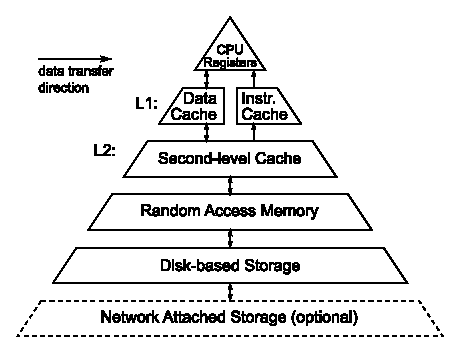
\includegraphics{memhier}
\caption{Schematic depiction of the memory hierarchy}\label{fig-memhier}
\end{figure}

In the memory hierarchy, every next level of storage is both significantly slower and significantly larger than the one above it and with increasing memory sizes, the block size increases as well. Table \ref{tab-memhier} gives an overview of typical memory sizes, block sizes, and access times. The values for the (general purpose) registers, L1 cache and L2 cache are those for the Pentium M processor as given in \cite{intel-opt}; other values are approximate.

\begin{table}
\begin{center}
\begin{tabular}{ l l l l }
\hline
\textbf{Type} & \textbf{Total Size} & \textbf{Block Size} & \textbf{Access Time} \\
\hline
Registers  &   32 bytes & 4 bytes & 1 cycle \\
L1 Cache   &   32 KB    & 64 bytes & 3 cyles \\
L2 Cache   &    1 MB    & 64 bytes & 9 cycles \\
RAM        &   ~2 GB    & 1 KB     & 50-100 cycles \\
Disk       & ~300 GB    & 4 KB     & 5,000-10,000 cycles \\
\hline
\end{tabular}
\caption{Sizes and access times of various types of storage}
\label{tab-memhier}
\end{center}
\end{table}

To conclude: the memory model used in real computer systems is quite a bit more complex than the uniform memory model assumed. Given this reality, the performance of many existing algorithms and data structures can be improved by taking the existence of a memory hierarchy into account. This has prompted research into new memory models that are more realistic. We will consider three classes of data structures and algorithms, depending on the assumptions that are made about the environment in their definition:
\begin{list}{}{}
\item \textbf{Cache-unaware} data structures and algorithms are designed with the traditional uniform memory model in mind, without considering the existance of a memory hierarchy, and may therefore not perform optimally in practice.
\item \textbf{Cache-aware} (or \textbf{cache-conscious}) data structures and algorithms are designed to perform optimally in the external memory model (,described below) but require parametrization with some or all properties of the cache layout (such as block size or cache memory size).
\item \textbf{Cache-oblivious} data structures and algorithms are designed to perform optimally in the cache-oblivious model (which will also be described below) which does not allow parametrization with properties of the cache layout.
\end{list}

Plenty of cache-unaware and cache-aware data structures have been developed and these are also widely used in practice. Altough some research has been done for cache-oblivious data structures, they are seldom used in practice. The main contribution of this paper is to give some insight in the practical merit of cache-oblivious data structures.

\subsection{External Memory Model}
One of the earliest models to take the differences in memory access cost into account is the external memory model, described by Aggarwal and Vitter \cite{aggarwal1988ioc}. They make a distinction between internal memory (which is limited in size) and external memory (which is virtually unlimited). The external memory is subdivided into blocks of a fixed size and only entire blocks of data can be transferred between the two memories; additionally, consecutive blocks can be transfered at reduced cost (so-called bulk transfer). Although Aggarwal and Vitter focus on magnetic disk as a storage medium for external memory, the model can be generalized to apply to every pair of adjacent levels in the memory hierarchy. In that case, the possibility of bulk transfer may have to be dropped.

We will call algorithms that are designed to minimize the number of transfers in a two-level memory hierarchy ``cache-aware'' (as opposed to traditional ``cache-unaware'' algorithms) or ``cache-conscious''. These algorithms typically rely on knowledge of the block size to achieve optimal performance.

\subsection{Hierarchical Memory Model}
The external memory model has the limitation that it only describes two levels of storage, while we have seen that in practice the memory hierarchy contains more than just two levels. Even though the external memory model can be used to describe any pair of adjacent levels, a particular algorithm can only be tuned to one. Aggarwal, Alpern, Chandra and Snir \cite{aggarwal1987mhm} addressed this shortcoming by introducing a hierarchical memory model in which the cost of accessing a value at specific memory address is described by a non-decreasing function of this address, which means that accessing data at higher addresses can be slower than at lower addresses. This more closely resembles a real memory hierarchy, but assumes that the application has full control over which data is placed where, which is usually not the case in practice, making their model of little use in the design and evaluation of practical algorithms.

\subsection{Cache-Oblivious Memory Model}
A different approach to generalizing the external memory model was taken by Prokop \cite{prokop1999coa} who proposed the cache-oblivious model, which consists of an infinitely large external memory and an internal memory of size M which operates as a cache for the external memory. Data is transferred between the two in aligned data blocks of size B. In contrast with the hierarchical memory model, the application does not have explicit control over the transfering of blocks between the two memories. Instead, it is assumed that an optimal cache manager exists which minimizes the number of block transfers over the execution the program. Additionally (and in contrast with the external memory model) the values of parameters like M and B are not known to the application, so they cannot be used explicitly when defining algorithms and datastructures. Of course, analysis in terms of memory transfers does involve these parameters, so the number of memory transfers performed is still a function of M and B (and other parameters relevant to the problem).

Algorithms that perform optimally in this model are called ``cache-oblivious'' and they distinguish themselves from cache-aware algorithms in that they cannot rely on knowledge of the block size or other specific properties of the cache configuration. The key advantage of this class of algorithms is that they are implicitly tuned to all levels in the memory hierarchy at once. It has been conjectured that these algorithms may therefore perform better than algorithms that are tuned to a specific level in the hierarchy only.

Demaine gives an introduction into the cache-oblivious memory model and an overview of a selection of cache-oblivious data structures and algorithms \cite{demaine2002coa}. He also motivates the simplifications made in the cache-oblivious memory model, such as the assumption of full cache associativity and an optimal replacement policy.

% Copy and shorten introduction from proposal
% -> Motivate research into cache-efficient algorithms
% -> Move "classification" subsection describing three models to front
% -> Describe each of the three models
% -> Introduce three data structures:
%     - note that hash tables have poor locality of reference
%     - note that btrees have good locality of reference but require pagesize
% -> Finally, present goal of the research (incorporate "Research Questions" in
% proposal)

% Marielle suggested:
%  - give the "standard" memory model an explicit name
%    (isn't "cache-unaware" enough?)
%  - move examples of cache oblivious data structures to front
%  - mention examples of cache unaware and cache aware algorithms
%    (at least Btree, tries and hash tables are mentioned)

% Note explicitly that cache-oblivious algorithms are relatively complex
% resulting in higher constant consts, so that the main question is wether
% the improved locality of reference compensates for the overhead incurred.

\section{Contributions}
Several cache-oblivious data structures and algorithms have been proposed. Complexity analysis shows that the proposed solutions are asymptotically optimal. However, in software engineering practice we are not only interested in computational complexity, but also in the practical performance of data structures and algorithms. Indeed, many algorithms that have suboptimal computational complexity are actually widely used because they perform well in practice (for example, sorting algorithms like Quicksort and Shell sort) and the converse is true as well: some algorithms, although theoretically sound, are unsuitable for practical use because of greater memory requirements, longer execution time, or difficulty of implementation (for example: linear-time construction of suffix arrays is possible, but in practice slower alternatives are often prefered that are easier to implement and require less memory).

This raises the question whether cache-oblivious data structures are actually preferable to traditional data structures in practice. To determine if cache-oblivious data structures have practical merit, empirical performance data is required, which is scarce as existing research has focused mainly on theoretical analysis. This paper addresses the question by reporting on the performance of newly implemented (but previously described) cache-oblivious data structures and their traditional counterparts (both cache-aware and cache-unaware data structures).

\section{Related Work}
Many data structures and algorithms have been analyzed in the cache-oblivious model. Several new data structures and algorithms have been developed that perform optimally in this mo\-del as well. Prokop presents asymptotically optimal cache-oblivious algorithms for matrix transposition, fast Fourier transformation and sorting \cite{prokop1999coa}.

Bender, Demaine and Farach-Colton designed a cache-oblivious data structure that supports the same operations as a B-tree \cite{bender2005cob} achieving optimal complexity bounds on search and nearly-optimal bounds on insertion. Later, Bender, Duan, Iacono and Wu simplified the data structure \cite{bender2004lpc} while preserving the supported operations and complexity bounds and adding support for finger searches. The latter data structure consists of a sparse array (stored in a linear amount of memory) with a static search tree in van Emde Boas layout (named for similarity to a different data structure proposed by van Emde Boas et al. \cite{vanemdeboas1976dai}).

Askitis and Zobel \cite{askitis2005ccc} propose a way to make chained hash tables more cache-efficient, by storing bucket contents in contiguous memory instead of using a linked list. This means buckets have to be resized on insertions and deletions, but their experiments show a performance gain over traditional methods (especially when the hash table is heavily loaded).

Vitter presents a theoretical survey of algorithms evaluated in a parallel disk model \cite{vitter2001ema}, which is a refinement of the external memory model described by Aggarwal and Vitter, but only allows parallel transfer of multiple blocks from different disks, which is more realistic. Unfortunately, his survey lacks empirical results.

Olsen and Skov evaluated two cache-oblivious priority queue data structures in practice \cite{olsen2002coa} and designed an optimal cache-obli\-vious priority deque. Their main result is that although the cache-obli\-vious data structures they examined make more efficient use of the cache, they do not perform better than traditional priority queue implementations.


\section{Methods}
In order to gather emperical data, the research approach must be made more concrete. We will need to limit ourselves to a specific class of data structures, since algorithms and data structures offering different functionality cannot be compared in a meaningful way. Furthermore, we will need to select a proper scenario in which the data structures are evaluated, as conclusions on the practical merit of the data structures depend on the degree to which the test scenario is realistic.

Furthermore, we will need to define what practical performance is. We will measure two properties: primarily, the total running time of our test application, and secondarily the memory used. The rationale for selecting these metrics is that if the data structures perform identical functions and plenty of memory is available, the only observable difference in running a program using different data structures will be the run time. Memory use is of secondary interest because in practice memory may be limited, which would preclude the use of certain data structures that require a lot of memory to function.

\subsection{State Space Search}
As the test application, that of a state space search has been chosen. This is a
suitable scenario for two reasons. First, it is commonly used as a practical
component of formal methods for software verification, and therefore good
algorithms are of great practical significance. Second, as we will explain
below, the performance of state space search algorithms depends for a large
part on the performance of the data structures that are used to implement
them; therefore, research into efficient data structures is of particular
interest to this application.

State space search is used to verify the correctness of software programs. For
this purpose, programs are first modeled using a formal language, that is also
used to specify properties of the program that should hold during its
execution. An executing program can be in a (possibly infinite) amount of states,
one of which is usually designated the \emph{initial state}. If a transition
from one state to another is possible (according to the rules of the formal
language used) the latter state is said to be a \emph{successor state} of the
former.
Generating the successors of a particular state is also called
\emph{expanding} the state. Of course, the model must include some form of
non-determinism to allow more than one successor to exist for a single state.
In practice, this non-determinism usually comes from processes that execute in
parallel, where the precise interleaving of the (observed) execution of
instructions in these processes is non-deterministic, unless synchronization
primitives (such as channels, semaphores, atomic execution blocks, et cetera)
are used to enforce a particular ordering.

The set of all states reachable by transitions from the initial state is called
the \emph{state space} of a model, and it is the goal of a state space search
algorithm to generate all of these states, in order to check that desired
properties hold in all of them. For this approach it is often required that
the state space be finite (for obvious reasons).

\begin{program}
\begin{verbatim}
Queue queue = new Queue;
Set generated = new Set;
queue.insert(initial_state);
while (!queue.empty()) {
    State state = queue.extract();
    for (State s : successors(state)) {
        if (generated.contains(s) == false) {
            generated.insert(s);
            queue.insert(s);
        }
    }
}
\end{verbatim}
\caption{Pseudo-code for a simple state search algorithm.}
\label{prog-search}
\end{program}

The outline of a state space search algorithm is given in Program
\ref{prog-search}. Note that in addition to the initial state and a function
to generate successors, a queue and a set data structure are used. The queue
holds states that have been generated but not yet expanded and is used to
determine what state to expand next. The set holds all states that have been
generated so far and is used to prevent a single state from being expanded
more than once.

Depending on how states are inserted and extracted from the queue, the search
may be breadth-first (meaning that all states that are reachable in $N$ steps
from the initial state are expanded before any states that require more than
$N$ steps) or depth-first (meaning that states that are generated most recently
by the successor function are expanded first). In the first case, the queue
operates by a first-in first-out principle, while in the second case the queue
works in a last-in first-out (stack) principle. In general, breadth-first
search requires a much larger queue capacity than depth-first search.

From the pseudo-code it is clear that the state space search algorithm does not
accomplish much by itself; instead, the real work is done by the successor
function and the queue and the set datastructures. Queues can easily be
implemented efficiently (adding and removing states takes O(1) time).
The efficiency of the successor function depends on the execution model used,
but is typically linear in the number of states produced. In practice,
therefore, the bottleneck of the algorithm is the set data structure.

\subsection{Experimental Framework}

% Describe (globally) what to measure: execution time
% - NIPS VM
% - SPIN model checker
% - Promela-to-NIPS compiler

For our experimental framework, we need a collection of formal models that are
representative of those typically used for formal verification, and a way to
execute them. For the first part, we have looked at Spin \cite{spin}, a widely
used model checking tool. Spin uses a custom modeling language, called
PROMELA, to specify models and comes with a collection of example models that
are suitable for our experiment.

For the execution of these models we will use NIPS VM \cite{weber2007evm}, a
high-performance virtual machine for state space generation that is easily
embeddable in our framework. Although the NIPS VM only executes bytecode in a
custom format, a PROMELA compiler is also available to generate the required
bytecode from the Spin models.\cite{nips} The NIPS VM is prefered to over the
Spin tools because it was designed to be embedded in other programs and as
such is more easily integrated in our framework.

The NIPS VM represents program state as a binary string; the size of the state
depends on the number of active processes in the program, and is typically in
the order of a few hundred bytes.

\subsection{Data Structures}
% TODO: copy motivation for reimplementation from proposal
% TODO: specify required operations (insert&contains)
% TODO: note that all data structures require contiguous memory
%       (except the Bender set)
% TODO: note use of mmap for automatic storage management

\subsubsection{Hash Table Implementation}
Hash tables are widely used as a fast (O($1$)) data structure especially when
used for in-memory storage. In its simplest form, a hash table consists of an
index array (the \emph{index}) with a fixed number of slots. A \emph{hash
function} is used to map key values onto slot numbers. If the slot for a value
is empty, it may be inserted there. Queries for the existance of an element in
the hash table similarly see if the queried value is stored at its designated
slot.

Note that if we insert several different values, some values may map to the
same slot, which is problematic if each slot can only store one value. There
are a lot of different ways to resolve this collision problem; we use
\emph{separate chaining} which means that slots do not store values directly,
but instead each slot stores a pointer to a singly-linked list of values that
map to that slot. This particular implementation technique is well-suited to
the scenario where values may have different sizes (as the slots only need to
store a fixed-size pointer and not a variable-size value) and maintains
relatively good performance when the number of values stored exceeds the size
of the index array \cite{sedgewick1998ac}.

% TODO: picture?

Our hash table implementation uses a fixed size index which must be specified
when creating the hash table, as this simplifies the implementation
considerably. The index is stored at the front of the file, after which values
are simply appended in the order in which they are added. Note that we do not
support removing elements from the hash table, which means we do not have to
deal with holes that would otherwise occur in the stored file. For our
experiments the FNV-1a hash function \cite{noll2004fnv} is used (modulo the
size of the index) to map values to slots.

\subsubsection{B-tree Implementation}
The B-tree data structure was first proposed by Bayer and McCreight
\cite{bayer1970oam} and is widely implemented and often described in
textbooks. Our implementation is based on the description by Kifer, Bernstein
and Lewis \cite{kifer2006dsa}.

B-trees are similar to other search tree data structures. A defining property
is that they organize data in pages of a fixed size, each containing several
values, which makes them especially useful for purposes of on-disk storage
where reading and writing data in a few large blocks is relatively cheap
compared to accessing several smaller blocks.

B-trees work by keeping as much values as possible, in order, in a single
page. Pages are ordered in a tree structure, where interior nodes store
pointers to child nodes. Pointers originate at a pair of adjacent values,
and point to a subtree containing only values that fall in between those
values.

When a new value does not fit in the page where it is to be inserted,
the page is split into two pages; the median value from the old page is
moved to the parent page, and two new pages (containing the values less
than respectively greater than the median) are created. When the top-most
page needs to be split, a new (empty) top-level page is created and the height
of the B-tree is increased by one.

B-trees are well suited to storing variable length values, as pages can
store many values as long as the combined size of the values and pointers
does not exceed the pagesize.

% TODO: picture and description

Note that there is no obvious way to store values that are larger than the
size of a single page. Production-quality implementations handle this case
separately, but our implementation does not support this scenario and
requires stored values to be smaller than the pagesize. Additionally,
deletion of items has not been implemented.

\subsubsection{Cache-Oblivious Dictionary Implementation}
% TODO: reference (if not included earlier)

% sparse array
% configurable density parameter
% note that equal division of gaps over all windows is important
%   (and note the problems with the "old" behaviour)
% binary search tree index
% van Emde Boas lay-out
% special optimization on insertion (note that it's not described by Bender)

\subsection{Measurements}
% Describe how performance was measured
%  (mock set implementation; times/sizes subtracted)

% Describe data set used; per model:
%   average state size
%   total size
%   ratio of insertions/queries

% Note that state size depends on number of processes

The following models are used for benchmarking:
\begin{itemize}
\item\verb#eratosthenes# is a parallel implementation of the sieve
of Eratosthenes which is used to find prime numbers upto a given maximum.
It has a single parameter $N$: only integers from 2 to $N$ (exclusive) are
tested. A new process is created for every prime number found, and as a result
the state space can only by exhaustively searched for relatively small values
of $N$ (e.g. $N < 40$). Because processes are dynamically created, state size
also varies during execution.

\item\verb#leader2# is a leader election algorithm with a configurable number
of processes competing for leadership ($N$). Since a constant number of
processes will be created and these processes cannot make progress until all
of them are created, almost all states have the same size.

\item\verb#peterson_N# is a Peterson's solution to the multi-process mutual
exclusion problem (using global variables instead of channels for
communication) with a configurable number of processes ($N$). The processes
are created atomically, so the state size is constant after initialization.

% mobile1
% pftp
% snoopy
% sort

% TODO: table of models with parameters, 

\end{itemize}

\section{Results}
% Present results!
% Tables, graphs, etc.
% What to include:
%   per program:     transitions/states graph
%   per program/set: 
%
%   

\section{Discussion}
% Explain results, draw conclusions.

\section{Conclusion}
% Repeat findings.

\bibliographystyle{plain}
\bibliography{paper}
\end{document}
